\documentclass[a4paper]{article}

\usepackage[T1]{fontenc}
\usepackage[utf8]{inputenc}
\usepackage{mlmodern}

%\usepackage{ngerman}	% Sprachanpassung Deutsch

\usepackage{graphicx}
\usepackage{geometry}
\geometry{a4paper, top=15mm}

\usepackage{subcaption}
\usepackage[shortlabels]{enumitem}
\usepackage{amssymb}
\usepackage{amsthm}
\usepackage{amsmath}
\usepackage{mathtools}
\usepackage{braket}
\usepackage{bbm}
\usepackage{graphicx}
\usepackage{float}
\usepackage{yhmath}
\usepackage{tikz}
\usepackage{scratch}
\usetikzlibrary{patterns,decorations.pathmorphing,positioning}
\usetikzlibrary{calc,decorations.markings}

\usepackage[backend=biber, sorting=none]{biblatex}
\addbibresource{cite.bib}

\usepackage[framemethod=TikZ]{mdframed}

\tikzstyle{titlered} =
    [draw=black, thick, fill=white,%
        text=black, rectangle,
        right, minimum height=.7cm]


\usepackage[colorlinks=true,naturalnames=true,plainpages=false,pdfpagelabels=true]{hyperref}
\usepackage[parfill]{parskip}
\usepackage{lipsum}

\usepackage{tcolorbox}
\tcbuselibrary{skins,breakable}

\pagestyle{myheadings}

\colorlet{colexam}{black}
\newcounter{definition}
\newtcolorbox[use counter=definition]{mydef}[1]{
    empty,
    title={\textbf{Definition~\thetcbcounter}~~(\textit{#1})},
    attach boxed title to top left,
    fontupper=\sl,
    boxed title style={
        empty,
        size=minimal,
        bottomrule=1pt,
        top=1pt,
        left skip=0cm,
        overlay=
            {\draw[colexam,line width=1pt]([yshift=-0.4cm]frame.north
        west)--([yshift=-0.4cm]frame.north east);}},
            coltitle=colexam,
            fonttitle=\normalfont,
            before=\par\medskip\noindent,
            parbox=false,
            boxsep=-1pt,
            left=0.75cm,
            right=3mm,
            top=4pt,
            breakable,
            pad at break*=0mm,
            vfill before first,
            overlay unbroken={
                \draw[colexam,line width=1pt]
                ([xshift=0.6cm, yshift=-0.5pt]frame.south
                west)--([xshift=0.6cm,yshift=-1pt]frame.north west)
                --([xshift=0.6cm]frame.south west)--([xshift=-13cm]frame.south east); },
            overlay first={
                \draw[colexam,line width=1pt]
                ([xshift=0.6cm, yshift=-0.5pt]frame.south
                west)--([xshift=0.6cm,yshift=-1pt]frame.north west)
                --([xshift=0.6cm]frame.south west); },
            overlay last={
                \draw[colexam,line width=1pt]
                ([xshift=0.6cm, yshift=-0.5pt]frame.south
                west)--([xshift=0.6cm,yshift=-1pt]frame.north west)
                --([xshift=0.6cm]frame.south west)--([xshift=-13cm]frame.south east); }
}
\newcounter{theorem}
\newtcolorbox[use counter=theorem]{theorem}{
    empty,
    title={Theorem ~\thetcbcounter},
    attach boxed title to top left,
    fontupper=\sl,
    boxed title style={
        empty,
        size=minimal,
        bottomrule=1pt,
        top=1pt,
        left skip=0cm,
        overlay=
            {\draw[colexam,line width=1pt]([yshift=-0.4cm]frame.north
        west)--([yshift=-0.4cm]frame.north east);}},
            coltitle=colexam,
            fonttitle=\bfseries,
            before=\par\medskip\noindent,
            parbox=false,
            boxsep=-1pt,
            left=0.75cm,
            right=3mm,
            top=4pt,
            breakable,
            pad at break*=0mm,
            vfill before first,
            overlay unbroken={
                \draw[colexam,line width=1pt]
                ([xshift=0.6cm, yshift=-0.5pt]frame.south
                west)--([xshift=0.6cm,yshift=-1pt]frame.north west)
                --([xshift=0.6cm]frame.south west)--([xshift=-13cm]frame.south east); },
            overlay first={
                \draw[colexam,line width=1pt]
                ([xshift=0.6cm, yshift=-0.5pt]frame.south
                west)--([xshift=0.6cm,yshift=-1pt]frame.north west)
                --([xshift=0.6cm]frame.south west); },
            overlay last={
                \draw[colexam,line width=1pt]
                ([xshift=0.6cm, yshift=-0.5pt]frame.south
                west)--([xshift=0.6cm,yshift=-1pt]frame.north west)
                --([xshift=0.6cm]frame.south west)--([xshift=-13cm]frame.south east); }
}
\newcounter{lemma}
\newtcolorbox[use counter=lemma]{lemma}{
    empty,
    title={Lemma~\thetcbcounter},
    attach boxed title to top left,
    fontupper=\sl,
    boxed title style={
        empty,
        size=minimal,
        bottomrule=1pt,
        top=1pt,
        left skip=0cm,
        overlay=
            {\draw[colexam,line width=1pt]([yshift=-0.4cm]frame.north
        west)--([yshift=-0.4cm]frame.north east);}},
            coltitle=colexam,
            fonttitle=\bfseries,
            before=\par\medskip\noindent,
            parbox=false,
            boxsep=-1pt,
            left=0.75cm,
            right=3mm,
            top=4pt,
            breakable,
            pad at break*=0mm,
            vfill before first,
            overlay unbroken={
                \draw[colexam,line width=1pt]
                ([xshift=0.6cm, yshift=-0.5pt]frame.south
                west)--([xshift=0.6cm,yshift=-1pt]frame.north west)
                --([xshift=0.6cm]frame.south west)--([xshift=-13cm]frame.south east); },
            overlay first={
                \draw[colexam,line width=1pt]
                ([xshift=0.6cm, yshift=-0.5pt]frame.south
                west)--([xshift=0.6cm,yshift=-1pt]frame.north west)
                --([xshift=0.6cm]frame.south west); },
            overlay last={
                \draw[colexam,line width=1pt]
                ([xshift=0.6cm, yshift=-0.5pt]frame.south
                west)--([xshift=0.6cm,yshift=-1pt]frame.north west)
                --([xshift=0.6cm]frame.south west)--([xshift=-13cm]frame.south east); }
}

\newcommand{\eps}{\varepsilon}
\usepackage[OT2,T1]{fontenc}
\DeclareSymbolFont{cyrletters}{OT2}{wncyr}{m}{n}
\DeclareMathSymbol{\Sha}{\mathalpha}{cyrletters}{"58}

\markright{Popović\hfill Seminar\hfill}


\title{University of Vienna\\
\vspace{1cm}Seminar:\\Joint RICAM Seminar\\
\vspace{0.5cm}
Summary of talk by Otmar Scherzer
}
\author{Milutin Popovic}


\begin{document}
\maketitle
\tableofcontents
\section{Sheet 1}
\subsection{Exercise 1}
Let $X \subseteq \mathbb{R}^{n}$ be an nonempty convex set and
$f:\mathbb{R}^{n} \to \mathbb{R}$ a convex function. Show that every local
minimum of $f$ w.r.t. $X$ is a global minimum of $f$ w.r.t. $X$.
\newline

Let $x^{*} \in X$ be the local minimum of $f$ w.r.t. $X$. Then there is an
$\varepsilon$-ball $B_{\varepsilon}(x^{*}) = \{x \in X:\ \|x^{*}- x\|\le
\varepsilon\}$ such that $f(x^{*}) \le f(x)$ for all $x \in
B_\varepsilon(x^{*}) \cap X$. Now suppose $x^{*}$ is not a global minimum
then there is a $x_{0} \in X$ such that $f(x_{0}) < f(x^{*})$. Since $X$ is
convex there is a line connecting $x_{0}$ and $x^{*}$ in $X$. This line has
elements of the form
\begin{align}
    L = \left\{\left( 1-\lambda \right)x_0 - \lambda x^{*}:\ \lambda \in[0,1]
    \right\}
    \subseteq X
\end{align}
Now for all $z \in L$ with $z = (1-\lambda)x_0 - \lambda x^{*}$ ($\forall
\lambda \in [0, 1]$) it holds that
\begin{align}
    &\|x^{*}- (1-\lambda)x_0 - \lambda x^{*}\| \le \varepsilon \\
    &(1-\lambda) \|x^{*}- x_{0}\| \le \varepsilon \; \Rightarrow \; \lambda
    \simeq 1
\end{align}
and
\begin{align}
    f\left( \left( 1-\lambda \right)x_{0} +\lambda x^{} \right)
    &\le \lambda f(x^{*}) + (1-\lambda) f(x_0)\\
    &< \lambda f(x_0) + (1-\lambda)f(x_0)\\
    &= f(x_0)
\end{align}
This means that we found a $\tilde{x} = \lambda x^{*} - (1-\lambda)x_0 \in
B_\varepsilon(x^{*})$ such that $f(\tilde{x}) < f(x^{*})$ which is a
contradiction since $x^{*}$ is a local minimum in $B_\varepsilon(x^{*})$.
This means that $x^{*}$ is a global minimum of $f$ w.r.t $X$.
\subsection{Exercise 2}
Let $X \subseteq \mathbb{R}^{n}$ be a nonempty, $x_0 \in X$. Show that
\begin{enumerate}
    \item $T_X(x_0)$ is a nonempty closed cone
    \item If $X$ is convex, then $T_X(x_0) = \text{cl}\left( \bigcup_{\lambda
        \ge 0 } \lambda \left( X - x_0 \right)  \right)$
    \item If $X$ is convex then $\left( T_X(x_0))^{*} = - N_X(x_0) \right) $
\end{enumerate}
The statements will be proven in chronological order. Starting with $1.$ the
Bouligand tangent cone to $X$ is defined as
\begin{align}
    T_X(x_0) = \{d \in \mathbb{R}^{n}: \exists (x^{k})_{k\ge 0}\subset X, \exists
    (t_k)_{k\ge 0}\searrow 0 :\ \frac{x^{k} -x_0}{t_k}\to d\}
\end{align}
Now $T_X(x_0)$ is nonempty since for $x^{k} = x_0$ for all $k$ and a sequence $t_k =
\frac{1}{k}$ we have
\begin{align}
    \frac{x^{k}-x_0}{t_k} \to 0 \in T_X(x_0)
\end{align}
To show that $T_X(x_0)$ is closed, consider a sequence $(d_k)_{k\ge 0}\subset
T_X(x_0)$ with convergence point $d \in \mathbb{R}^{n}$. To show that it is closed we
need to show that $d \in T_X(x_0)$. So for all $d_n \in (d_k)_{k\ge 0}
\subset T_X(x_0)$ there exists a sequence $(x^{n,k})_{k\ge 0} \subset X$ and
a sequence $(t_{n, k})_{k\ge 0}$ with $t_{n, k} \searrow 0$ as $k \to
\infty$ such that
\begin{align}
    &\frac{x^{n,k}-x_0}{t_{n,k}} \to d_n \;\;\; \forall n\ge 0,\\
    &\text{and}\nonumber\\
    &\lim_{n\to \infty}\lim_{k \to \infty}\frac{x^{n,k}-x_0}{t_{n,k}} = d.
\end{align}
Then there exist $K_\varepsilon$ and $N_\delta$ for $\varepsilon,\delta >0$
such that
\begin{align}
    &\|d_k - d\|\le \varepsilon \;\; \forall k\ge K_\varepsilon,\\
    &\|\frac{x^{n,K_\varepsilon}-x_0}{t_{n,K_\varepsilon}} -
    d_{K_\varepsilon}\| \le \delta \;\; \forall n \ge N_\delta.
\end{align}
To conclude the proof consider
\begin{align}
    &\|\frac{x^{N_\delta,K_\varepsilon}-x_0}{t_{N_\delta,K_\varepsilon}} -
    d\|\\
    &= \|\left(\frac{x^{N_\delta,K_\varepsilon}-x_0}{t_{N_\delta,K_\varepsilon}} -
    d_{K_\varepsilon}\right) + \left( d_{K_\varepsilon} - d\right) \|\\
    &\le \varepsilon + \delta
\end{align}
Meaning that $d \in T_X(x_0)$.
Then
$T_X(x_0)$  is really a cone because $\forall d \in T_X(x_0)$ and $\lambda
>0$ we have that $\lambda d \in T_X(x_0)$ by the choice $t_{k,\lambda}=
\frac{1}{\lambda}t_k$
\begin{align}
    \frac{x^{k}- x}{t_{k,\lambda}} = \lambda \frac{x^{k}-x_0}{t_k}\to
    \lambda d \in T_X(x_0)
\end{align}
For number 2 additionally $X$ is a convex set. And by
definition of a cone $\bigcup_{\lambda \ge 0}(X-x_0)$ is a cone. And the
union of convex sets is also convex the set
$\text{cl}\left(\bigcup_{\lambda\ge_0} \lambda(X-x_0 ) \right)$ is also.
convex.
For number 3 we simply calculate
\begin{align}
    -\left( T_X(x_0) \right)^{*}
    &= -\{s \in R^{n}: s^{T}d \ge 0 \forall d \in T_X(x_0)\}\\
    &= \{s \in R^{n}: s^{T}d \le 0 \forall d \in T_X(x_0)\}\\
    &= \{s \in R^{n}: s^{T}(x-x_0) \le 0 \forall x \in X\}
\end{align}
Since $forall x \in X$ there exists an appropriate sequence converging to $x$
subjected to the tangent cone elements.
\subsection{Exercise 3}
Let $X \subseteq \mathbb{R}^{n}$ be nonempty and $\text{dist}_X: \mathbb{R}^{n}
\to \mathbb{R}$, with $\text{dist}_X(y) = \inf \{\|y-x\|: x\in X\}$. Then consider the
directional derivative of a function $f: \mathbb{R}^{n}\to \mathbb{R}$ at
direction $d$ at $x_0 \in \mathbb{R}^{n}$
\begin{align}
    f'(x_0; d) = \lim_{t \downarrow 0} \frac{f(x_0 + t d) - f(x_0)}{t}
\end{align}
Show that if $X \subseteq \mathbb{R}^{n}$ is nonempty and convex then the
tangent cone can be written as
\begin{align}
    T_X(x_0) = \{d \in \mathbb{R}^{n}:\; \left( \ \text{dis}t_X
    \right)'(x_0;d) = 0\}.
\end{align}
First we note
\begin{align}
    (\text{dist}_X)'(x_0;d) = \lim_{t \downarrow 0} \frac{\text{dist}_X(x_0+t
    d)}{t} = 0,
\end{align}
is true for all $x_0 + t d \in X$. Since $X$ is convex we have that
\begin{align}
    T_X(x_0) &= \text{cl}\left( \bigcup_{\lambda}\left( X-x_0 \right)  \right)
    \\
             &= \text{cl}\left( \{\lambda (x - x_0): x\in X, \lambda \ge 0\}  \right)
\end{align}
Then $(\text{dist}_X)'(x_0;d) = 0$ holds only for vectors of the form
$d = \lambda (x - x_0)$, $\lambda \ge 0$ and $x \in X$.
\subsection{Exercise 4}
We consider the general constrained optimization problem
\begin{align}
    \text{min}\quad & f(x),\\
    \text{s.t.}\quad & g_i(x) \le 0, i=0,\ldots,m\nonumber\\
    &h_j(x) = 0, j=0,\ldots,p\nonumber\\
    & x \in \mathbb{R}^{n}\nonumber
\end{align}
for $f, g_i, h_j: \mathbb{R}^{n}\to \mathbb{R}$, $i=0,\ldots,m$ and
$j=0,\ldots,p$ continuously differentiable. Let $x_0$ be a feasible element
of the problem and
\begin{align}
    X_{\text{lin}} := \{ x \in \mathbb{R}^{n}:\quad
    &g_i(x_0) + \nabla g_i(x_0)^{T}(x-x_0), i=0,\ldots,m\\
    &h_j(x_0) + \nabla h_j(x_0)^{T}(x-x_0), j=0,\ldots,p\}.
\end{align}
Show that $T_\text{lin}(x_0) = T_{X_\text{lin}}(x_0)$.
\newline
For the reminder
\begin{align}
    T_{\text{lin}}(x_0) := \{ d \in \mathbb{R}^{n}:\quad
    &\nabla g_i(x_0)^{T}d, \forall i \in \mathcal{A}(x_0)\\
    &\nabla h_j(x_0)^{T}d, j=0,\ldots,p\},
\end{align}
where $\mathcal{A}(x_0) = \{i=i,\ldots,m:g_i(x_0) = 0\}$. First we show that
$X_\text{lin}$ is convex then we can use the second part of exercise 2. So
for all $x, y \in X_{\text{lin}}$ we need to show that $z=(1-\lambda)x
\lambda y \in X_{\text{lin}}$, this is done by checking the conditions
\begin{align}
    &\nabla g_i(x_0) + \nabla g_i(x_0)^{T} (z-x_0)\\
    &=\nabla g_i(x_0) + \nabla g_i(x_0)^{T} ((1-\lambda)x + \lambda y-x_0)\\
    &=\nabla g_i(x_0) + \nabla g_i(x_0)^{T} (x-\lambda x + \lambda y-x_0)\\
    &=\nabla g_i(x_0) + \nabla g_i(x_0)^{T} (x-x_0)
    + \nabla g_i(x_0)^{T}(-\lambda x + \lambda y)\\
    &\le \lambda \nabla g_i(x_0)^{T}(-x + y) \qquad (\lambda \ge 0 )\\
    &\le \nabla g_i(x_0)^{T}(- x + y + x_0 - x_0) + g_i(x_0)
    -g_i(x_0)\\
    &=-\nabla g_i(x_0) - \nabla g_i(x_0)^{T} (x-x_0)
    + \nabla g_i(x_0) + \nabla g_i(x_0)^{T} (y-x_0)\\
    &\le 0
\end{align}
and similarly for $h_j$
\begin{align}
    &\nabla h_j(x_0) + \nabla h_j(x_0)^{T} (z-x_0)\\
    &=\nabla h_j(x_0) + \nabla h_j(x_0)^{T} ((1-\lambda)x + \lambda y-x_0)\\
    &=\nabla h_j(x_0) + \nabla h_j(x_0)^{T} (x-\lambda x + \lambda y-x_0)\\
    &=\nabla h_j(x_0) + \nabla h_j(x_0)^{T} (x-x_0)
    + \nabla h_j(x_0)^{T}(-\lambda x + \lambda y)\\
    &= \lambda \nabla h_j(x_0)^{T}(-x + y)\\
    &= \lambda \nabla h_j(x_0)^{T}(- x + y + x_0 - x_0) + \lambda h_j(x_0)
    -\lambda h_j(x_0)\\
    &=\lambda\left(-\nabla h_j(x_0) - \nabla h_j(x_0)^{T} (x-x_0)
    + \nabla h_j(x_0) + \nabla h_j(x_0)^{T} (y-x_0)\right)\\
    &= 0
\end{align}
Thereby $X_{lin}$ is convex and
\begin{align}
    T_{X_\text{lin}}(x_0) = \bigcup_{\lambda \ge 0 }\lambda \left(
    X_\text{lin} - x_0 \right) .
\end{align}
Additionally $T_{lin}(x_0)$ is a polyhedral so per definition
\begin{align}
    T_\text{lin}(x_0) = \bigcup_{\lambda \ge 0 }\lambda \left( X_\text{lin} -
    x_0 \right)
\end{align}
\subsection{Exercise 5}
Let $g: \mathbb{R}^{2} \to \mathbb{R}^{4}$ with
\begin{align}
    g(x, y) =
    \begin{pmatrix}
        \pi - 2x\\
        -y - 1\\
        2x - 3\pi\\
        y - \sin(x)
    \end{pmatrix}.
\end{align}
and
\begin{align}
    X = \{(x,y) \in \mathbb{R}^{2}: g(x,y) \leqq 0\}.
\end{align}
The set $X$ has the following constrains on $x, y$
\begin{align}
    \pi - 2x \le 0 \; \Rightarrow x \ge \frac{\pi}{2}\\
    -y - 1 \le 0 \Rightarrow y \ge -1\\
    2x - 3\pi \le \Rightarrow x \le \frac{3\pi}{2}\\
    y - \sin\left( x \right) \le 0 \Rightarrow y \le 1,
\end{align}
meaning $x \in [\frac{\pi}{2}, \frac{3\pi}{2}]$ and $y \in [-1, 1]$.
The tangent cones of $X$ w.r.t $x_1 = (\frac{\pi}{2}, 1)^{T},
x_2=(\pi,0)^{T}$ and $x_3 = (\frac{3\pi}{2}, -1)^{T}$ are
\begin{align}
    T_X(x_1) = \{(0, -\lambda)^{T}, (\lambda, 1)^{T}: \lambda > 0\} \\
    T_X(x_2) = \{\lambda(\cos(x), \sin(x))^{T}, (\lambda, 1)^{T}: \lambda > 0\} \\
    T_X(x_3) = \{(-\lambda, 0)^{T}, (0, \lambda)^{T}: \lambda > 0\}
\end{align}
Graphically it represents the following
\begin{figure}[H]
    \centering
    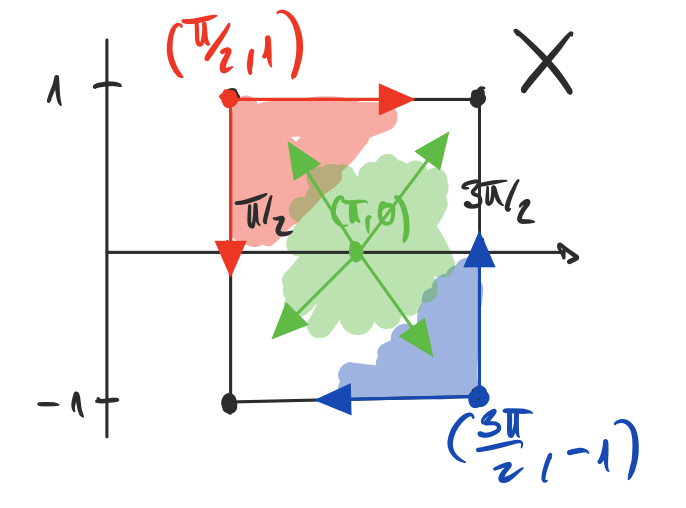
\includegraphics[width=0.4\textwidth]{./build/pics/sesh1_ex5.png}
    \caption{Graphical representation of $X$ and tangent cones $T_X(x_i)$, $i=1, 2,
    3$}
    \label{fig:}
\end{figure}
Then we look at the linearized tangent cones $T_\text{lin}(x_i) = \{d\in \mathbb{R}^{2}:
\nabla g_i(x_i)^{T} d \le 0 \forall i \in \mathcal{A}(x_i)\}$. First we
calculate the gradients of entries of $g$
\begin{align}
    \nabla g_1(x, y) = (-2 ,0)^{T}\qquad \nabla g_2(x,y) = (0, -1)^{T}\\
    \nabla g_3(x, y) = (2 ,0)^{T}\qquad \nabla g_4(x,y) = (-\cos(x), 1)^{T}
\end{align}
then for all $j  \in \{ 1, 2, 3, 4\} $ and $i \in \{1, 2, 3\}$ we check if
$g_j(x_i) \le 0$ and construct $\mathcal{A}(x_i)$ and then find $d$ subjected
to the condition.
For $x_1$ we have
\begin{align}
    g_1(x_1) = 0,\;\;
    g_2(x_1) \neq 0,\;\;
    g_3(x_1) \neq 0,\;\;
    g_4(x_1) = 0 \;\;\\
    \Rightarrow \mathcal{A}(x_1) = \{1, 2\}
\end{align}
Then
\begin{align}
    T_{\text{lin}}
    &= \{d \in \mathbb{R}^{2} : (0, 1)d \le 0, (-2, 0)d \le 0\}\\
    &=\{(\lambda, 0)^{T} , (0, -\lambda)^{T}: \lambda >0 \}
\end{align}
For $x_2$ we have
\begin{align}
    g_1(x_1) \neq 0,\;\;
    g_2(x_1) \neq 0,\;\;
    g_3(x_1) \neq 0,\;\;
    g_4(x_1) \neq 0 \;\;\\
    \Rightarrow \mathcal{A}(x_1) = \{4\}
\end{align}
Then
\begin{align}
    T_{\text{lin}}
    &= \{d \in \mathbb{R}^{2} : (1, 1)d \le 0\}\\
    &=\{(-\lambda, \lambda)^{T} , (\lambda, -\lambda)^{T}, (-\lambda, 0)^{T}, (0,
    -\lambda)^{T}: \lambda >0 \}
\end{align}
For $x_3$ we have
\begin{align}
    g_1(x_1) \neq 0,\;\;
    g_2(x_1) = 0,\;\;
    g_3(x_1) = 0,\;\;
    g_4(x_1) = 0 \;\;\\
    \Rightarrow \mathcal{A}(x_1) = \{2, 3, 4\}
\end{align}
Then
\begin{align}
    T_{\text{lin}}
    &= \{d \in \mathbb{R}^{2} : (0, -1)d \le 0, (2, 0)d\le 0, (0, 1)d \le 0\}\\
    &=\{(-\lambda, 0)^{T}: \lambda >0 \}
\end{align}
We conclude that $T_{X_\text{lin}}(x_i) = T_{\text{lin}}(x_i)$ only for $i=1$.
\subsection{Exercise 6}
Let $A \in \mathbb{R}^{n \times  m}$ and $b \in \mathbb{R}^{m}$. Prove using
the strong duality theorem of linear optimization that the following
statements are equivalent
\begin{enumerate}
    \item The system $Ax = b$ has a solution $x \leqq 0$
    \item It holds $b^{T}d \ge 0$ for all $d \in \mathbb{R}^{m}$ with $A^{T}d
        \leqq 0$
\end{enumerate}
we show that $1$ is equivalent to $\neg \exists d \in R^{m}: Ad \le 0$
and $b^{T}d > 0$. Consider the following primal dual
\begin{align}
    \text{max}\quad & 0^{T}x\\
    \text{s.t.:}\quad & Ax=b\nonumber\\
                      &x\leqq 0\nonumber\\
    \text{and}\nonumber\\
    \text{min}\quad & b^{T}d\\
    \text{s.t.:}\quad & Ad\le 0\nonumber\\
                      &d \in R^{m}\nonumber\\
\end{align}
Consider a solution of $Ax = b$ such that $x \ge 0$. This means that the
primal is true, so there exists an optimal solution since $0^{T}x=0$ then $0$
must be this primal optimal. By the duality $0$ must be the optimal of the
dual problem, which means $b^{T}d =0 $  so there is no $d \in \mathbb{R}^{m}:
b^{T}d >0$.\newline
On the other hand $\neg \exists d \in \mathbb{R}^{m}: Ad \le 0$ and $b^{T}d
>0$ so $\forall d' \in \mathbb{R}^{m}$ we have that $Ad' > 0$ or $b^{T}d \le
0$ such that $b^{T}d \leq 0 $ for all $d \in \mathbb{R}^{m}$. So we can
conclude that there exists a solution because the primal has at least one
feasible $x \in \mathbb{R}^{m}: Ax = 0, x\geqq 0$. Thereby the two statements
above are equivalent.

\end{document}


